\chapter{Theory}
\label{cha:theory}

This chapter introduces background and related work.

\section{Background}
\label{sec:background}

In this section, we give background to the tackled problem and outline the theory behind our approach.
Sections \ref{sec:visualsearch} and \ref{sec:activevision} provide perspective to the problem from neuroscience and machine perception respectively.
Section \ref{sec:deeplearning} overviews the theory behind function approximation with neural networks, and some common neural network architectures.
Section \ref{sec:reinforcementlearning} summarizes the foundations of reinforcement learning and deep reinforcement learning.

\subsection{Visual Search and Attention}
\label{sec:visualsearch}

The perceptual task of searching for something in a visual environment is usually referred to as \textit{visual search}~\cite{wolfe_visual_2010}.
The object or feature that is being searched for is referred to as the \textit{target}, and the other objects or features in the environment as \textit{distractors}.
This task has been studied extensively in psychology and neuroscience.

Two big limitations of performance in visual search are processing power, and limited observability.
Processing high-dimensional sensory input like images is expensive, and environments are often too large and complex to view all at once.
An observer that searches a scene for targets has to direct its \textit{visual attention} to one region at a time.
Humans scan environments by directing their gaze (\textit{overt attention}) and shifts of attention in the current visible region (\textit{covert attention})~\cite{itti_computational_2001}.
While covert attention tends to be reactionary, overt attention usually integrates more features over time.
In this work we focus specifically on the former, moving the gaze to bring targets into view.

Humans control overt attention through both eye movements and head movements.
Eye movement is almost instant between locations, and the cost of directing attention with eye movements is constant regardless of distance.
This is not true for head movements, and in general not true for robotic systems:
movements induced by motors tend to come at a cost that is proportional to the distance moved, both in time and energy.
The cost of directing overt attention means that there is a need to do so strategically.

If the searched environment is a random field, visual search is akin to a random process~\cite{nakayama_situating_2011}.
Experiments in humans have shown that search in featureless environments is consistent with random walk with no memory.
Optimal search algorithms in such environments would be exhaustive, such as those found in coverage path planning~\cite{galceran_survey_2013}.
Humans have also been shown to use the history of observations to improve visual search efficiency. 
Simple memory mechanisms, like some inhibition-of return mechanism~\cite{itti_computational_2001} that prevents searching visited locations twice, improve search time in random fields considerably.

Natural environments are in fact seldom completely random, but instead tend to exhibit some structure.
When finding targets, there is usually something about this structure that can be utilized to improve search performance.
Such regularities can learned from past experience and used during future searches.
Improvements in human search performance have been measured when certain locations have higher probabilities of containing targets~\cite{eckstein_visual_2011,wolfe_five_2017}.
Furthermore, if targets usually co-occur with other visible elements they tend to be easier to find~\cite{eckstein_visual_2011,wolfe_five_2017}.

\subsection{Active Vision and Object Search} 
\label{sec:activevision}

Much of past and present research in machine perception involves a passive observer which samples and perceives images from a fixed distribution.
Animal perception, in contrast, is active -- we do not only see, but also decide where to look.
In the \textit{active vision} paradigm, an the observer has some control of its sensory input.~\cite{aloimonos_active_1988}

Active vision, and \textit{active perception} in general, is a problem of intelligent data acquisition.
An active observer must control its sensory inputs to constrain the interpretation of its environment.
One of the difficulties of active perception problems is that they are scene and context dependent.
A thorough understanding of the data acquisition parameters and the goal of the visual processing is needed.~\cite{bajcsy_active_1988}

%While certain tasks are necessarily active vision tasks, there is an argument to be made that active vision is a means to solve the task more effectively.
%Indeed, active vision systems have several computational advantages over passive ones~\cite{aloimonos_active_1988}.
%Furthermore, an active learning system acquires the samples to learn from itself select more informative samples to learn from than a passive one.

%Bajcsy, Aloimonos and Tsotsos~\cite{bajcsy_revisiting_2018} state that

%\begin{quote}
%    An agent is an active perceiver if it knows why it wishes to sense,
%    and then chooses what to perceive, and determines how, when and where to achieve that perception.
%\end{quote}

In active vision, searching for objects with a camera in unknown environments is referred to as \textit{object search} or \textit{active object localization}.
A searching observer has to both recognize and localize its targets, while controlling its sensory input.
To search effectively, it must also model its environment and perform path planning.~\cite{chen_active_2011}

Solving the object search problem optimally involves determining a sequence of camera controlling actions that maximizes the probability of finding the target while satisfying a cost constraint.
The state of the searcher is uniquely determined by the control parameters of the camera.
Actions that adjust these parameters and adjust the observed region come at some cost in time or energy.
Finally, the agent has some prior knowledge of the probability of targets which it updates after each observation.
Finding an optimal solution in three dimensional search spaces has been shown to be NP-complete, necessitating approximate solutions.~\cite{ye_complexity-level_2001,andreopoulos_theory_2009}

\subsection{Deep Learning}
\label{sec:deeplearning}

Deep learning is a family of techniques in which hypothesis are represented as computation graphs with tunable weights.
The computation graphs are inspired by biological neurons in the brain and are referred to as \textit{neural networks}.
Deep neural networks consist of \textit{nodes} arranged in \textit{layers}: one input layer, zero or more hidden layers and one output layer.
Each layer receives an input \textit{representation}~\cite{bengio_representation_2013} from the previous layer and outputs a transformed representation to the next layer.
Given some input, a neural network optimizes its output representation with regard to some criterion.
Usually, a loss function \(\mathcal{L}\) is minimized by updating the weights \(\mathbf{w}\) of the network with some variant of \textit{gradient descent} with learning rate \(\alpha\):

\begin{equation}
    \mathbf{w} \leftarrow \mathbf{w} - \alpha \nabla_\mathbf{w} \mathcal{L}(\mathbf{w}) 
\end{equation}

The only requirement on the functions computed by each node is that it is differentiable.
As long as this holds, layers can be stacked arbitrarily and the gradients can be computed with the chain rule.
This way, errors in the output can be passed back through the network (\textit{back-propagation}) and used to update the weights.~\cite{russell_artificial_2021,goodfellow_deep_2016}

The architecture of a neural network imposes some bias onto the learning that its expected to be useful for generalizing to unseen samples.
We now describe three neural network architectures that will be used in this work.

\subsubsection{Feedforward Neural Network}

A feed-forward neural network, also known as a multi-layer perceptron (MLP)~\cite{goodfellow_deep_2016}, only has connections in one direction.
Each node in the network receives inputs from its predecessors and outputs the result of a function of those inputs.
The output \(y\) of each node is usually computed by taking the weighted sum of its inputs \(x\) and applying some non-linear function

\begin{equation}
    y_j = g_j(\mathbf{w}_j^T \mathbf{x}),
\end{equation}

where \(y_j\) is the output of node \(j\), \(g_j\) is a non-linear \textit{activation function}, \(\mathbf{w}_j\) is the vector of weights leading into node \(j\), and \(\mathbf{x}\) is the vector of inputs to the node.
By convention, each layer also has some \textit{bias} that allows the total weighted input to \(g_j\) to be non-zero even when the outputs from the previous layer are zero.
The bias is included as an extra input \(x_0\) fixed to 1, and an extra tunable weight \(w_{0,j}\).
The non-linearity ensures that a network with at least two layers can approximate any continuous function.~\cite{russell_artificial_2021}

\subsubsection{Convolutional Neural Network}

Convolutional neural networks (CNNs) contain spatially local connections.
They have patterns of weights, called \textit{kernels}, that are replicated across units in each layer.
With some input vector \(\mathbf{x}\) of size \(n\) and a vector kernel \(\mathbf{k}\) of size \(l\), the (discrete) convolution operation \(\mathbf{z} = \mathbf{x} \ast \mathbf{k}\) is defined as

\begin{equation}
    z_i = \sum_{j=1}^l k_j x_{j+1-\frac{l+1}{s}},
\end{equation}

where \(s\) is the \textit{stride}.
This operations can be generalized up to more than one dimension, such as 2 dimensions for images and 3 dimensions for volumes.
With multiple input channels, kernels are stacked into a \textit{filter}.
The outputs of each kernel are then summed over, giving one output channel per filter.

There are several advantages to using CNNs for structured input data where neighboring values are correlated.
Kernels are smaller than the input, which means that fewer parameters have to be stored.
These \textit{sparse interactions} give CNNs reduced memory requirements,
as well as improved statistical and computational efficiency.

Furthermore, the same parameters are also used for more than one function in the CNN. \textit{Parameter sharing} across input locations mean that layers in a CNN have \textit{equivariance} to translation. 
The output of one kernel is the same regardless of the input location.
This property of CNNs is useful for images where similar features may be useful regardless of their location in the input.~\cite{goodfellow_deep_2016}

\subsubsection{Recurrent Neural Network}
\label{sec:rnn}

Recurrent neural networks (RNNs) extend feed-forward networks by allowing cycles in the computation graph.
Each cycle has a delay so that some \textit{hidden state} from the previous computation is used as input to the current computation.
A recurrent layer with input \(\mathbf{x}_t\), output \(\mathbf{y}_t\) and hidden state \(\mathbf{z}_t\) is defined by

\begin{align}
    \begin{split}
        \mathbf{z}_t &= f_\mathbf{w}(\mathbf{z}_{t-1}, \mathbf{x}_t) \\
        \mathbf{y}_t &= g_y(\mathbf{W}_{z,y}, \mathbf{z}_t),
    \end{split}
\end{align}

where \(f_\mathbf{w}\) is the update process for the hidden state and \(g_y\) is the activation function for the hidden layer.
This model can be turned into a feed-forward network over a sequence of input vectors \(\mathbf{x}_1, \dots \mathbf{x}_T\) and observed outputs \(\mathbf{y}_1, \dots, \mathbf{y}_T\) by \textit{unrolling} it for \(T\) steps. The weights are shared across all time steps. This means that RNNs can operate on inputs of arbitrary lengths.
The hidden state is used as a summary of all previous items in the sequence.
Thus, RNNs make a Markov assumption.~\cite{russell_artificial_2021}

In practice, conventional RNNs struggle with learning long-term dependencies.
During back-propagation, gradients can tend to zero for long sequences, something known as the vanishing gradient problem~\cite{goodfellow_deep_2016}.
An architecture that addresses this issue is long short-term memory (LSTM)~\cite{hochreiter_long_1997}.
LSTMs include a \textit{memory cell} \(c\) in the hidden state that is copied from time step to time step, and three soft \textit{gating units} that govern the information flow in the hidden state update process \(f\). This makes LSTMs particularly useful for learning over long sequences.

\subsection{Reinforcement Learning}
\label{sec:reinforcementlearning}

Reinforcement learning (RL)~\cite{sutton_reinforcement_2018} is a subfield of machine learning concerned with learning from interaction how to achieve a goal.
This section introduces the fundamental concepts of RL.

\subsubsection{Partially Observable Markov Decision Processes}
\label{sec:pomdp}

The problem of learning from interaction to achieve some goal is often framed as a Markov decision process (MDP).
A learning \textit{agent} interacts continually with its \textit{environment}.
The agent takes the \textit{state} of the environment as input, and select an \textit{action} to take.
This action updates the state of the environment and gives the agent a scalar \textit{reward}.
It is assumed that the next state and reward depend only on the previous state and the action taken.
This is referred to as the \textit{Markov} property.~\cite{kaelbling_planning_1998}

In an MDP, the agent can perceive the state of the environment with full certainty.
For many problems, including the one we consider here, this is not the case.
The agent can only perceive a partial representation of the environment's state.
Such a process is referred to as a partially observable Markov decision process (POMDP).
A POMDP is formally defined as a 7-tuple \(\left\langle \mathcal{S}, \mathcal{A}, \mathcal{T}, \mathcal{R}, \Omega, \mathcal{O}, \gamma \right\rangle\), where

\begin{itemize}
    \item \(\mathcal{S}\) is a finite set of states,
    \item \(\mathcal{A}\) is a finite set of actions,
    \item \(\mathcal{T}: \mathcal{S} \times \mathcal{A} \rightarrow \Pi(\mathcal{S})\) is a state-transition function,
    \item \(\mathcal{R}: \mathcal{S} \times \mathcal{A} \rightarrow \mathbb{R}\) is a reward function,
    \item \(\Omega\) is a finite set of observations,
    \item \(\mathcal{O}: \mathcal{S} \times \mathcal{A} \rightarrow \Pi(\Omega)\) is an observation function, and
    \item \(\gamma \in [0, 1]\) is a discount factor.
\end{itemize}

Assume that the environment is in state \(s_t \in \mathcal{S}\), and the agent selects action \(a_t \in \mathcal{A}\).
Then, \(T(s_t, a_t, s_{t+1})\) is the probability of ending in state \(s_{t+1}\) and \(r_t = R(s_t, a_t)\) is the expected reward gained by the agent.
The agent also receives an observation \(o_t \in \Omega\) with probability \(\mathcal{O}(s_{t+1}, a_t, o_t)\).~\cite{kaelbling_planning_1998}
Figure \ref{fig:pomdp} illustrates the interaction between agent and environment.

\begin{figure}
    \centering
    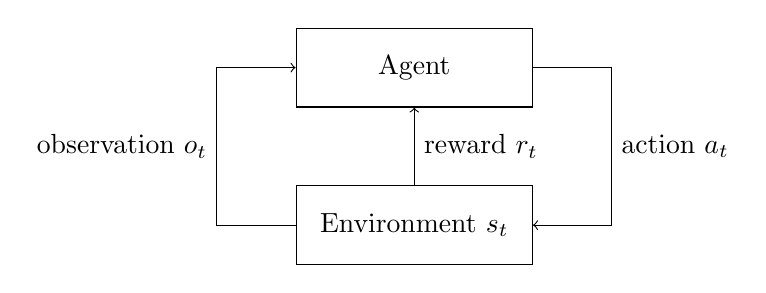
\begin{tikzpicture}[node distance=2cm]
    \tikzstyle{block} = [rectangle,minimum width=3cm,minimum height=1cm,text centered,draw=black,fill=white]
    \node (agent)[block]{Agent};
    \node (environment)[block,below of=agent]{Environment \(s_t\)};
    \draw [->] (agent.east) -- ++(1cm,0) -- node [anchor=west]{action \(a_t\)} ++(0,-2cm) -- (environment.east);
    \draw [->] (environment.north) -- node [anchor=west]{reward \(r_t\)} (agent.south);
    \draw [->] (environment.west) -- ++(-1cm,0) -- node [anchor=east]{observation \(o_t\)} ++(0,+2cm) -- (agent.west);
\end{tikzpicture}
    \caption[Partially observable Markov decision process]{Interaction between agent and environment in a partially observable Markov decision process.}
    \label{fig:pomdp}
\end{figure}

The agent and environment interact over a sequence of discrete time steps \(t = 0, 1, \dots, T\), giving rise to an \textit{episode} of length \(T\).
At each time step \(t\), the goal of the agent is to select the action that maximizes the expected \textit{discounted return}:

\begin{equation}
    \mathbb{E} \left[ \sum_{k=0}^T \gamma^{k-t-1} r_k \right]
\end{equation}

Since the agent receives partial observations of the environment's state, it has to act under uncertainty.
Planning in a POMDP is undecidable, and solving one is often computationally intractable.
Approximate solutions are more common, where the agent usually maintains an internal \textit{belief state}~\cite{kaelbling_planning_1998} which is acts on.
The belief state summarizes the agent's previous experience and is therefore dependent on the full \textit{history} of actions and observations.
It does not need to summarize the whole history, but generally only the information that helps the agent maximize the expected reward.
From here on we will use the belief state and the environment state \(s\) interchangeably. 
% Sutton page 467 is better, contains latent state assumption

\subsubsection{Policies and Value Functions}
\label{sec:policy-value}

The behavior of the agent is described by its \textit{policy}.
A policy \(\pi\) is a mapping from perceived environment states to actions.
Policies are often stochastic and specify probabilities for each action, with \(\pi(a|s)\) denoting the probability of taking action \(a\) in state \(s\).~\cite{sutton_reinforcement_2018}

Most RL solutions methods also approximate a \textit{value function}.
A value function \(V_\pi\) estimates how good it is to be in a state.
The value function \(V_\pi(s)\) is the expected (discounted) return when starting at state \(s\) and following policy \(\pi\) until the end of the episode.
There are two common alternative value functions:
The \textit{quality function} \(Q_\pi(s,a)\) gives the value of state \(s\) under policy \(\pi\) where \(a\) is the first action taken.
Given a quality function, \textit{action-value} methods choose the action greedily at every state as \(arg\,max Q_\pi(s, a)\).
The \textit{advantage function} \(A_\pi(s, a)\) instead represents the relative advantage of actions, \(A_\pi = Q_\pi - V_\pi\).~\cite{sutton_reinforcement_2018}

For problems with large state and action spaces, it is common to represent value functions with \textit{function approximation}.
In such cases, it is common to encounter states that have never been encountered before.
This makes it important that the estimated value function can generalize from seen to unseen states.
With examples from the true value function, an approximation can be made with supervised learning methods.
We write \(\hat{V}(s,\mathbf{w}) \approx V_\pi(s)\) for the approximate value of state \(s\) with some weight vector \(\mathbf{w} \in \mathbb{R}^d\).~\cite{sutton_reinforcement_2018}

An alternative to action-value methods is to approximate the policy itself.
\textit{Policy gradient} methods learn a parametrized policy that select actions without a value function.
We denote a parametrized policy as \(\pi(a|s,\boldsymbol{\theta})\) with \(\boldsymbol{\theta} \in \mathbb{R}^{d^\prime}\) as the parameters to the policy.
The policy parameters are usually learned based on the gradient of some performance measure \(L(\boldsymbol{\theta})\).
As long as \(\pi(a|s,\boldsymbol{\theta})\) is differentiable with respect to its parameters, the parameters can be updated so as to optimize for the objective.~\cite{sutton_policy_1999}

Advantages of policy parametrization over action-value methods include stronger convergence guarantees~\cite{sutton_policy_1999} and more flexibility in parametrization~\cite{sutton_reinforcement_2018}.
However, less is known about if and how fast policy gradient methods converge to globally optimal policies~\cite{agarwal_optimality_2020}
In practice, value functions are often still used to learn the policy parameter, but they are not needed for action selection.
Such methods are called \textit{actor-critic} methods, with actor referring to the learned policy and critic referring to the learned value function.
In these cases, there might also be some overlap between the weights \(\mathbf{w}\) of the value function estimate and \(\boldsymbol{\theta}\) of the policy estimate. 

One important aspect of function approximation is its interplay with partial observability.
If there is a state variable that is not observable, as for partially observable environments,
then the parametrization can be chosen such that the approximate value does not depend on that state variable.
Because of this, function approximation is applicable to the partially observable case.~\cite{sutton_reinforcement_2018}

% {arulkumaran_survey_2017} also gives a good introduction to algorithms
% https://www.davidsilver.uk/wp-content/uploads/2020/03/intro_RL.pdf
% https://spinningup.openai.com/en/latest/spinningup/rl_intro2.html
% https://sites.ualberta.ca/~szepesva/rlbook.html

\subsubsection{Design Challenges}

% we can illustrate the challenges in terms of our problem

One of the challenges that arises in reinforcement learning is the exploration-exploitation trade-off.
An RL agent should \textit{exploit} knowledge gained from previous experiences and prefer actions that has yielded reward in the past.
It should also \textit{explore} in order to learn better actions to take in the future.
Agents that fail to both exploit and explore will lead to failure at the task, and striking a good balance between the two is non-trivial.~\cite{sutton_reinforcement_2018}

Another challenge is the design of reward signals.
For some tasks, like certain video games, the objective is simply to maximize the score obtained.
In this case there is an inherent reward signal and the agent achieves its task simply by maximizing this inherent signal.
Other times, we have a task we want the agent to solve and have to design a reward signal around that task.
Designing rewards is not straight-forward and can often have unintended effects~\cite{sutton_reinforcement_2018}.
Special care has to be taken to ensure that the reward encourages the desired behavior.

Here, the problem of \textit{sparse rewards} also comes into play.
The agent has to be reward frequently enough to allow it to achieve its goal once.
Often it has to incentivize it to achieve its goal efficiently, with multiple different starting conditions.
If rewards are too sparse, the agent may explore aimlessly and take too long to find achieve its goal.
If the received reward is temporally distant from the action that caused it, the agent may have difficulty connecting the two.
This is known as the \textit{credit assignment problem}~\cite{minsky_steps_1961}.

In practice, rewards are often designed through trial-and-error.
Through \textit{reward shaping}~\cite{mataric_reward_1994},
the reward is designed so as to guide the agent towards achieving its goal by giving additional rewards along the way.
Several iterations of a reward signal are tried until one yields expected and sufficient results.

\subsubsection{Deep Reinforcement Learning}

As mentioned in Section~\ref{sec:policy-value}, policies and value functions are often approximated.
Neural networks have good properties for function approximation and have been used for RL with success.
One early example is TD-Gammon~\cite{tesauro_temporal_1995}, a neural network trained with RL that reached expert Backgammon performance in 1995.

More recently, the successes of deep learning have bled over into the field of RL.
In 2015, Mnih et al.~\cite{mnih_human-level_2015} extend \cite{mnih_playing_2013} and introduce DQN, which combines deep neural networks with RL.
DQN successfully plays Atari games using only visual input.
It approximates the quality function \(q(s, a)\) with a CNN architecture, and selects actions greedily.
To incorporate some memory, images from the 4 previous time steps are stacked and used as input to the neural network.
The input is fed through three convolutional layers and a hidden fully connected layer, all with ReLU activation functions.
The output layer has one output for each valid action, representing Atari controller buttons.

DQN inspired many several follow-up works which use deep neural networks to approximate policy and/or value functions.
Such methods are often referred to as deep reinforcement learning (deep RL) methods.

\subsubsection{Proximal Policy Optimization}
\label{sec:ppo}

Proximal policy optimization (PPO)~\cite{schulman_proximal_2017} is a family of policy-gradient algorithms that have turned out to strike a good balance between simplicity, stability and ease of tuning while achieving strong results on several tasks~\cite{schulman_proximal_2017,henderson_deep_2018,cobbe_leveraging_2020,vinyals_grandmaster_2019,andrychowicz_what_2020}.

PPO alternates between sampling agent-environment interactions over \(T\) time steps and optimizing the policy using those interactions.
The parameters \(\boldsymbol{\theta}\) of the policy \(\pi\) are updated with the objective

\begin{equation}
    \mathcal{L}_\text{CLIP}(\boldsymbol{\theta}) = 
    \hat{\mathbb{E}}_t \left\lbrack \min(r_t(\boldsymbol{\theta}) \hat{A}_t, \text{clip}(r_t(\boldsymbol{\theta}),1-\epsilon, 1+\epsilon) \hat{A}_t \right\rbrack.
\end{equation}

The expectation \(\mathbb{\hat{E}}\) indicates the empirical average over a finite batch of samples collected under the old policy with parameters \(\theta_{\text{old}}\).
Here, \(r_t(\theta) = \frac{\pi(a_t | s_t, \boldsymbol{\theta})}{\pi(a_t | s_t, \boldsymbol{\theta}_{\text{old}})}\) and \(\hat{A}_t\) is an estimate 
of the advantage function.
The clip range \(\epsilon\) is used to clip the surrogate objective,
putting a pessimistic bound on the product of the probability ratio and the advantage estimate.
This in turn ensures that the size of the policy updates is limited.

In an actor-critic approach, the advantage is estimated over using a learned state value function \(V(s)\) as 

\begin{equation}
    \hat{A}_t = \delta_t + (\gamma\lambda) \delta_{t+1} + \dots + (\gamma\lambda)^{T-t+1} \delta_{T-1}
\end{equation}

where \(\delta_t = r_t + \gamma V(s_t+1) - V(s_t)\).
If the policy and value functions estimations share parameters, for example in a multi-headed neural network architecture, a loss function that combines the policy loss and the value function error term must be used.
It is also common to introduce an entropy bonus to ensure sufficient exploration.
The full PPO objective for an actor-critic approach is

\begin{equation}
    \mathcal{L}_t(\boldsymbol{\theta}) =
    \hat{\mathbb{E}}_t
    \left\lbrack
    \mathcal{L}_\text{CLIP}(\boldsymbol{\theta}) -
    c_1 \mathcal{L}_\text{VF}(\boldsymbol{\theta}) +
    c_2 S [\pi](s_t, \boldsymbol{\theta})
    \right\rbrack
\end{equation}

where the coefficients \(c_1\) and \(c_2\) are hyperparameters determining the impact of the value loss and entropy bonus,
\(S\) is an entropy bonus and \(\mathcal{L}_\text{VF}\) is a squared-error loss in the value output. Algorithm~\ref{alg:ppo} shows the steps of the PPO algorithm.

\begin{algorithm}
    \caption{Proximal Policy Optimization}
    \label{alg:ppo}
    \begin{algorithmic}
        \For{\(\text{iteration} = 1,2,\dots\)}
            \For{\(\text{actor} = 1,2,\dots,N\)}
                \State \(\text{run policy } \pi_{\theta_\text{old}} \text{ for } T \text{ time steps}\)
                \State \(\text{compute advantage estimates } \hat{A}_1, \dots \hat{A}_T\)
            \EndFor
            \State \(\text{optimize } \mathcal{L} \text{ wrt } \theta, \text{ with } K \text{ epochs and mini-batch size } M \leq NT\)
            \State \(\theta_{\text{old}} \leftarrow \theta\)
        \EndFor
    \end{algorithmic}
\end{algorithm}

\section{Related Work}
\label{sec:relatedwork}

Works that consider tasks that are related to searching for targets in unknown environments can be found in several fields under many names.
In this section we survey some of the more relevant ones, focusing on those that employ RL methods.

\subsection{Search with Reinforcement Learning}

There are several rigorous attempts to implement robotic object search systems using non-learning methods.
Forssén et al.~\cite{forssen_informed_2008} implement a mobile robot that searches for specific objects within a cluttered environment.
Their robot explores by moving towards unexplored regions and looks around to identify potential objects.
Each objects is examined from several perspectives and ranked by probability of being the queried object.
Shubina and Tsotsos~\cite{shubina_visual_2010} model the search problem as in \cite{ye_complexity-level_2001}, and solve with a greedy action selection strategy.
They do not take environment appearance into account, and rely on prior knowledge of target distribution being provided as a spatial probability map.
Some works also take appearance and semantics of the environment into account to search more efficiently~\cite{aydemir_search_2011,aydemir_active_2013}.
%Meger et al.~\cite{meger_curious_2008} describe a system that performs object recognition in realistic scenarios\dots

These systems solve more complex tasks than the one we consider, such as handling multiple target object categories and navigating in obstructed environments.
However, they are also restricted by their reliance on human knowledge to act well in their environments.
While reinforcement learning is not among the more traditional solution methods for active vision tasks~\cite{chen_active_2011},
learning systems that are less dependent on expert knowledge have the potential to be more generally applicable.

\subsubsection{Sequential Visual Attention}

Minut and Mahadevan\cite{minut_reinforcement_2001} propose an sequential model of selective visual attention for visual search tasks.
An agent is tasked with finding a particular object in a scene
A policy for controlling a fixed pan-tilt-zoom camera is learned using reinforcement learning.
The goal of the agent is to aim the camera at the region where a target is most likely to be found.
It has to decide where to fixate next based on visual information only.
Despite being limited to a single environment, this is an early example of visual search modelled as an RL problem.

Mnih et al.~\cite{mnih_recurrent_2014} take inspiration from visual attention and foveated vision found in humans and propose to use a similar mechanism for computer vision tasks.
Applying a CNN to a large images can be expensive, as the complexity scales linearly with the number of images pixels.
They propose a recurrent model that extracts information from images by adaptively selecting a sequence of smaller regions to process at high resolution.
At each time step, the agent receives an image observation of the environment.
Through actions, the agent selects a limited region of this observation to view in high resolution.
It is given a reward that is dependent on the task the agent should perform.
It can access this image via a bandwidth-limited sensor which it focuses on a limited region.
The agent maintains an internal state using an LSTM layer.
Though the model is not differentiable, it is trained using RL with a policy gradient method.
The authors evaluate the agent for image classification and a game-like task.
They find that the model outperforms a similar convolutional architecture for cluttered object classification tasks.
This is attributed to its ability to focus its attention on important regions.

\subsubsection{Active Object Detection}

In computer vision, \textit{object detection} is the task of detecting semantic objects of a certain class in images.
Detecting an object entails \textit{recognizing} that it is present in an image, and \textit{localizing} it by determining its bounding box.
State of the art object detection use deep learning techniques and usually involve a deep convolutional architecture to recognize objects~\cite{zhao_object_2019}.
For localization, a region proposal process considers the whole image and returns a set of bounding box candidates.
The object recognizer is then run on each region proposal.
Region proposals are akin to visual attention, as they limit the region of the image that is processed by the recognizer.

Although we do not focus on difficult recognition problems in this work, object localization is highly relevant.
The difference is that images in object detection are passively sampled - they are drawn from some distribution and all are independent.
Furthermore, the whole scene that is searched for objects is visible in the image.
In \textit{active object detection}, the analyzed images are instead chosen so as to help the detector perform its task better.

Caicedo and Lazebnik~\cite{caicedo_active_2015} propose to use deep reinforcement learning for active object localization in images where the object to be localized is fully visible.
An agent is trained to successively improve a bounding box using translating and scaling transformations.
They use a reward signal that is proportional to how well the current box covers the target object.
An action that improves the region is rewarded with +1, and given a punishment of -1 otherwise.
They find that this reward communicates more clearly which transformations keep the object inside the box and which take the box away from the target.
When there is no action that improves the bounding box, the agent may select an indication action (which would be the only action that does not give a negative reward) which resets the box.
This way the agent may select additional bounding boxes.
Each indication action modifies the environment by marking it so that the agent may learn to not select the same region twice.

A similar work by Ghesu et al.~\cite{ourselin_artificial_2016} present an agent for anatomical landmark detection trained with deep RL.
Different from \cite{caicedo_active_2015} is that the entire scene is not visible at once.
The agent sees a limited region of interest in an image, with its center representing the current position of the agent.
The actions available to the agent translate the view up, down, left and right.
A reward is given to the agent that is equal to the supervised relative distance-change to the landmark after each action.
Three datasets of 891 anatomical images are used.
The agent starts at random positions in the image close to the target landmark and is tasked with moving to the target location.
While achieving strong results (90\% success rate), the scenes and targets are all drawn from a distribution with low variance.
Most real-world search tasks exhibit larger variance than a population of anatomical images of the human body.

Chen and Gupta~\cite{chen_spatial_2017} use a spatial memory for context reasoning in object detection.
They argue that object detection systems require memory to perform well.
Furthermore, they pose that this memory should capture the spatial layout of the scene in order to model object-object relationships.
Their proposed memory remembers features and locations of past detections in an image and uses this to improve future ones.
A CNN is used to extract features from the memory and used together with the original image as input to a standard region proposal network.
The approach gives a small improvement over the standalone region proposal network.

\subsubsection{Visual Navigation}

Visual navigation is the process of determining a suitable path between a start point and destination point using visual input.
Visual navigation has been studied for use in both autonomous ground vehicles, where obstacles have to be avoided, as well as for unmanned aerial vehicles which typically don't have the problem of avoiding obstacles~\cite{bonin-font_visual_2008}.
The visual search problem can be considered analogous to a visual navigation in unrestricted environments.

In recent years, several works have used deep RL to solve various visual navigation tasks.
These have mostly been focused on learning navigation between two points in indoor environments,
where the goal is either specified as an image of a target object or indirectly as a distance from the agent's location.
There are several simulated environments for such tasks~\cite{kolve_ai2-thor_2019,xia_gibson_2018,savva_habitat_2019}.

Zhu et al.~\cite{zhu_target-driven_2017} create a model for target-driven visual navigation in indoor scenes with deep RL.
An observer is given a partial image of its scene as well as an image of the target object, and is tasked with navigating to the object in the scene with a minimal number of steps.
The agent moves forwards, backwards, and turns left and right at constant step lengths.
They use a reward signal with a small time penalty to incentivize task completion in few steps.
They compare their approach to random walk and the shortest path and achieve promising results.
This setup is quite similar to the one considered in this report, but the authors make a few assumptions that we do not.
They a set of 32 scenes, each of which contain a fixed number of object instances.
They focus on learning spatial relationships between objects in these specific scenes, and have scene-specific layers to achieve this.
Thus, while they show that they can adapt a trained network to a new scene, their approach is unable to zero-shot generalize to new scenes.

Ye et al.~\cite{ye_active_2018} propose an alternative architecture to \cite{zhu_target-driven_2017} which, in addition to an image of the camera view and the target object, uses the output of an object recognition module to select actions.
Specifically, the output of the localization component is fed as input.
This allows the agent to know if the target object is in view, and where.
The object recognition module is trained separately from the policy.
While requires a set of images of potential target objects labelled with their class and location, it also illustrates how object recognition can be offloaded to a separate module in reinforcement learning agents that benefit from such functionality.

Yang et al.~\cite{yang_visual_2018} propose to use semantic scene priors to improve navigation towards objects in unseen scenes.
The agent observes its environment through a camera.
Prior knowledge of spatial relations between objects types is encoded as a graph, which is encoded with a graph convolutional network.
Their agent is also told what object to look for in the form of a word embedding.
The encoded object graph and word embedding is used as input together with the camera image to an actor critic network that selects actions that navigate towards the target object.
As the agent collects experiences, it also updates its prior knowledge of spatial relationships between objects.
It is shown that prior knowledge encoded in such a way improves the agents ability to navigate to objects.

Mnih et al.~\cite{mnih_asynchronous_2016} use a recurrent policy with only RGB images to navigate in a labyrinth.
3D labyrinths are randomly generated, and an agent is tasked with finding objects in them.
The same architecture as in \cite{mnih_human-level_2015} is used, but with 256 LSTM cells after the final hidden layer.
At each episode, a maze is randomly generated with objects that give rewards then traversed scattered around.
They train the agent using an actor-critic approach and manage to get the agent to successfully navigate in unseen but similar environments.

Mirowski et al.~\cite{mirowski_learning_2017} propose a new approach to tackle a similar maze navigation problem as \cite{mnih_asynchronous_2016}.
They introduce a new architecture, that in addition to an image, also observes the reward, velocity and the action from the previous time step.
Observing the reward may help the agent learn features of desirable frames, but also limits the set of possible reward signals as the reward has to be present during testing.
As in \cite{mnih_asynchronous_2016}, the agent has a recurrent LSTM layer. 
The architecture is trained using an auxiliary depth prediction objective.
The authors argue that understanding the depth of the searched environment helps the agent navigate it better.
This agent is evaluated against three baselines on both static and randomly generated maze environments.
It is found that an agent that only receives image observations performs worse than one that also has an LSTM layer.
Adding the previous reward, action and velocity to the observations bring modest performance improvements.
The depth prediction is found to improve performance in all environments, indicating that the correct auxiliary task can help learning.

Dhiman et al.~\cite{dhiman_critical_2019} critically investigate deep RL for navigation, using a CNN and RNN architecture as in \cite{hausknecht_deep_2017} and \cite{mirowski_learning_2017}.
They ask whether deep RL algorithms are inherently able to gather and exploit environmental information for during navigation.
Experimentally, they find that an agent is able to exploit environment information when trained and tested on the same map.
When trained and tested on different maps, the agent does not seem to be able to exploit environment information to navigate more effectively.
The authors use relatively small training set of less than 1000 samples, but do not consider that their agents could have overfit this this set.
Finally, they find that the agent is not able to consistently find optimal navigation paths in seen environments when its starting position is randomized.

%These works all focus on navigation between points in a scene.
%Visual search is perhaps more akin to intelligent visual exploration.
%https://vision.cs.utexas.edu/projects/exploring-exploration/

\subsection{Memory Architectures}

A recurring theme in the related work above is the use of memory architectures.
In most cases where active sensing is involved, memory is a requirement for good performance.
As mentioned in Section \ref{sec:pomdp}, effective behavior in partially observable processes usually requires some form of memory.
Agents need to summarize the history of interactions with their environment for good action selection.
Works that don't use memory rely on either full observability, like \cite{caicedo_active_2015}, or low variance so that search can be done reactively, like \cite{ourselin_artificial_2016}.
Memory is intuitively important for the search task we consider here, as integrating features over time should lead to more efficient search strategies.

Anderson et al.~\cite{anderson_evaluation_2018} emphasize the importance of memory mechanisms that support the construction of rich internal representations of environments in navigation agents.
They argue that the nature of the internal representation is central to the study of embodied navigation.
Simple agents that are purely reactive and act on the sensory input at the current time step only work for simple tasks.
Simple memory mechanisms, like the frame stacking used in \cite{mnih_human-level_2015} can model velocity and work well in certain environments where reactive action is sufficient.
Once a task requires integration of features over longer time, more advanced memory is required.

Augmentations like recurrent update mechanisms add more potential.
Hausknecht and Stone~\cite{hausknecht_deep_2017} investigate the effects of adding memory in the form of a recurrent step to DQN in order to tackle POMDPs.
They use the same convolutional network as \cite{mnih_human-level_2015}, but only use the most recent frame as input and replace the hidden layer with a recurrent LSTM layer.
It is found that the agent is able to integrate information over time and achieves comparable performance to the original DQN agent.
Several other works use a recurrent step to solve tasks that require memory, like~\cite{mnih_recurrent_2014} and \cite{mnih_asynchronous_2016}.
General-purpose recurrent neural networks can in theory remember anything, but have practical issues like the the ones described in Section~\ref{sec:rnn}.
Furthermore, they might not be easily trained for all tasks.

Specialized memory architectures can provide better performance for their intended tasks.
Oh et al.~\cite{oh_control_2016} propose one such memory that can retain information over a fixed limited number of time steps.
During each time step, the agent encodes its observation and shifts it into the memory.
It also reads the memory using a soft attention~\cite{bahdanau_neural_2016} mechanism whose weights are determined by the encoded observation.
This way, the agent can recall information from the past that is useful to the present.
The authors evaluate this architecture in several visual navigation tasks, where image observations are encoded with a CNN.
In their tests, their memory architecture performs better than LSTM layers, and generalizes better to unseen environments.

LSTM is an example of a temporal memory -- it remembers information across time.
Several works propose the use of spatial memories rather than temporal ones.
In these works, the term spatial refers to the fact that they are addressed with a position in the environment.
Agents can use such memories to write and read structured information of their environment.
Parisotto and Salakhutdinov~\cite{parisotto_neural_2017} introduce a general-purpose spatial memory architecture.
They assume that the environment can be discretized into a set of positions.
The agent retains a feature map with one feature vector per position it can occupy in the environment.
At each time step, the agent reads the feature map from the previous time step and writes information to the slot for its current position.
This architecture is shown to outperform LSTM and the architecture in \cite{oh_control_2016} in several navigation tasks which require remembering over many time steps. Several similar architectures have been proposed~\cite{henriques_mapnet_2018,gupta_cognitive_2019,chaplot_object_2020}.

\subsection{Generalization and Inductive Bias}

In RL, generalization refers to an agents ability to act well in environments that have not been seen during training.
This is vital if RL is to be applied to real-world problems where conditions are diverse and unpredictable.
Agents have to be robust to such variations without being trained on them (\textit{zero-shot} policy transfer).
In the case of visual search, we want a system that can search in novel environments by generalizing from those seen during training.

While deep neural networks have proved to be effective function approximators for RL, they are also prone to \textit{overfitting}.
High-capacity models trained over a long time may memorize the distribution seen during training rather than general patterns.
While studied in supervised learning, overfitting and generalization has generally been neglected in deep RL~\cite{kirk_survey_2022}.
Training and evaluation stages are typically not separated.
Instead, the final return on the training environments is used as a measure of agent performance.
This results in agents that perform badly on environments that are only slightly different from those seen during training.

Zhang et al.~\cite{zhang_study_2018} study overfitting and generalization in deep RL.
With experiments, they show that RL agents are capable of memorizing training data, even when completely random.
When the number of training samples exceeds the capacity of the agent, they overfit to them.
When exposed to new but statistically similar environments during testing, test performance could vary significantly despite consistent training performance.
The authors argue that good generalization requires the \textit{inductive bias} of the algorithms to be compatible with the bias of the problems.
The inductive bias refers to a priori algorithmic preferences, like neural network architecture.
When comparing MLPs with CNNs, they find that MLPs tend to be better at fitting the training data are worse at generalizing.
When rewards are spatially invariant, CNNs generalize much better than MLPs.
The authors advocate for carefully designed testing protocols for detecting overfitting.
The effectiveness of stochastic-based evaluation depends on the properties of the task.
Agents could still learn to overfit to random training data. 
For this reason, they recommend isolation of statistically tied training and test sets.

In a similar spirit, Cobbe et al.~\cite{cobbe_quantifying_2019} construct distinct training and test sets to measure generalization in RL.
They find that agents can overfit to surprisingly large training sets, and that deep convolutional architectures can improve generalization.
Methods from supervised learning, like L2 regularization, dropout, data augmentation and batch normalization are also shown to aid with generalization.

Many current deep RL agents do not optimize the true objective that they are evaluated against,
but rather a handcrafted objective that incorporates biases to simplify learning.
Stronger biases can lead to faster learning, while weaker biases potentially lead to more general agents.
Hessel et al.~\cite{hessel_inductive_2019} investigate the trade-off between generality and performance from the perspective of inductive biases.
Through experimentation with common reward sculpting techniques, they find that learned solutions are competitive with domain heuristics like handcrafted objectives.
Learned solutions also seem to be better at generalizing to unseen domains.
For this reason, they argue for avoiding biases determined with domain knowledge in future research.

Cobbe et al.~\cite{cobbe_leveraging_2020} introduce a benchmark for sample efficiency and generalization in RL.
They make use of procedural generalization, dependent on a random seed, to decide many parameters of the initial state of the environment.
This forces agents to learn policies that are robust variation and avoid overfitting.
To evaluate sample efficiency of agents in the benchmark, they train and test on the full distribution of states.
To evaluate generalization, they limit the number of training samples and then test on held out levels.
When an episode ends, a new sample is drawn from the training set.
Agents may train for arbitrarily many time steps.
The number of training samples required to generalize is dependent on the particulars and difficulty of the environment.
The authors choose the training set size to be near the region when generalization begins to take effect.
Empirically they find that larger model architectures improve both sample efficiency and generalization.
Agents strongly overfit to small training sets and need many samples to generalize.
Interestingly, training performance improves as the training set grows past a certain threshold.
The authors attribute this to the implicit curriculum of the distribution of levels.

Kirk et al.~\cite{kirk_survey_2022} survey generalization in deep RL.
They distinguish between methods that try to generalize from training to testing sets by increasing their similarity, and those that attempt to handle their differences.
To handle differences between training and test sets, an agent's policy should rely only on features which will behave similarly in the training and testing context.
If the similarities between training and testing contexts are known, they can be encoded as inductive bias for stronger generalization.
When there is not specific inductive bias to encode, standard regularization can be used.
Finally, when we can not rely on specific inductive biases or standard regularization, we have to rely on learning the invariances from training and hope that these generalize to testing.

They further propose a formalism for collections of problems called contextual CMDPs.
A CMDP which is an MDP \(\mathcal{M}\) (or POMDP) where the state can be decomposed into \(s = \left\langle c, s' \right\rangle\),
where \(s \in \mathcal{S}\) is the underlying state and \(c \in \mathcal{C}\) is the \textit{context}.
The context takes the role of a seed and determines the sample drawn from the underlying distribution of task instances.
In a CMDP, separate train and test tasks can be defined by creating \(\mathcal{C}_\text{train} \subseteq \mathcal{C}\) and \(\mathcal{C}_\text{test} \subseteq \mathcal{C}\) such that \(\mathcal{C}_\text{train} \cap \mathcal{C}_\text{test} = \varnothing\).
It is argued that the only choice when evaluating generalization with procedurally generated environments is the training set size.
Evaluation has to be performed on the full distribution of (held out) contexts.

\subsection{Evaluation of Agents}
\label{sec:theory-evaluation}

A problem in state-of-the art deep RL is reproducibility.
There is often non-determinism, both in the methods and environments used.
Furthermore, many methods have intrinsic variance which can make published results difficult to interpret.
In some cases, training an algorithm in an environment twice can give learning curves that do not fall within the same distribution~\cite{henderson_deep_2018}.
This has meant that reproducing state-of-the-art deep RL results is difficult.
A common solution is to report average results and variance across multiple different runs.

However, the sample inefficiency of current deep RL algorithms together with the rise in popularity of more challenging benchmarks has led to long training times.
This has made it less feasible to measure performance over many training runs,
which in turn has led to a shift to only evaluating a small number of runs (\(N \leq 5\)) per task.~\cite{agarwal_deep_2022}
This is problematic, as several analyses indicate that as many as \(N = 20\) runs are required for statistically significant results~\cite{colas_how_2018,colas_hitchhikers_2019}.

Henderson et al.~\cite{henderson_deep_2018} investigate reproducibility methods in deep RL empirically, focusing on policy gradient methods.
They try to reproduce results in works with published code bases, and investigate how various modifications affect results.

They find that hyperparameters and the choice of network architecture for policy and value function approximation can affect performance significantly.
Furthermore, rescaling rewards can have a large effect, although it is difficult to predict how.
It is found that ReLU activations tend to perform best across environments and algorithms.
For PPO, the use of large networks may require changing other hyperparameters like learning rate.
Confidence bounds with sample bootstrapping is used to show that PPO is among the more stable algorithms.

For certain environments, learning curves can indicate successful optimization but the learned behavior may not be satisfactory.
It is therefore important to not only show returns, but also demonstrations of the learned policy in action.
Interestingly, implementation differences that are not reflected in publications can have a dramatic impact on performance.
It is therefore necessary to enumerate implementation details and package code bases with publications.
Performance of baseline experiments should also match original baseline publication code.

Finally, \cite{henderson_deep_2018} make the point that more emphasis should be placed on applying RL algorithms to real-world tasks.
It could be more useful to propose a set of tasks that an algorithm could be used for than to show performance on fictional tasks.

Anderson et al.~\cite{anderson_evaluation_2018} discuss problem statements and evaluation measures for embodied navigation agents, and make a set of recommendations.
A navigation agent should be equipped with a special action that indicates that it has concluded the episode.
The agent should be evaluated at the time this action is made, and not at some more favorable time step.
Proximity to a goal should be measured using geodesic distance, the shortest distance in the environment.
They recommend success weighted by (normalized inverse) path length (SPL) as the primary measure of navigation performance.
With \(N\) test episodes, SPL is computed as 

\begin{equation}
    \text{SPL} = \frac{1}{N} \sum_{i=1}^N S_i \frac{l_i}{\max(p_i, l_i)}
    \label{equ:spl}
\end{equation}

where \(S_i\) is a binary indicator of success,
\(l_i\) is the shortest path distance from the agent's starting position to the goal,
and \(p_i\) is the length of the path actually taken in the episode.
SPL takes the quality of the solution into account:
If 50\% of test episode are successful and the agent takes the optimal path in all of them, its SPL is 0.5.
By measuring SPL of human subjects, what is a good score can be calibrated.
